\RequirePackage[hyphens]{url}
\documentclass[sigchi]{acmart}
%% Include the standard set of goodies
\usepackage{amsmath,amssymb,amsfonts,amsthm} % Lots of useful math, symbols, etc.
\usepackage{comment}                         % Comment environment---nothing within is typeset
\usepackage{ifthen}                          % One of many approaches to simple conditionals when writing macros
\usepackage{minibox}                         % Alignment/frame-supporting wrapper around \vbox{\hbox{...}...\hbox{...}}
\usepackage{multirow}                        % Row-spanning table cells
\usepackage{suffix}                          % Macros with non-alphabetic suffixes (Requires e-TeX)
\usepackage{graphicx}                        % \includegraphics command to include images
\usepackage[hyphens]{url}                    % \url command
\usepackage{xargs}                           % \newcommandx command for defining commands with default args
\usepackage{hyperref}                        % Hyperlinks
\usepackage[capitalise]{cleveref}            % \cref for automatically using the right word for refs
\usepackage{hyphenat}                        % \hyp{} for line-wrappable hyphen, plus redefines \_ to be line-wrappable
\usepackage{subcaption}                      % \subcaption command for captioning subfigures
\usepackage{fancyvrb}                        % Verbatim environment: less brittle than \verb
\usepackage{xcolor}                          % colors!
\usepackage{supertabular}                    % supertabular environment: allows tables to flow to next page
\usepackage{xspace}                          % fixes space after text-only macros

% Proper english
\newcommand\ie{i.e.,\xspace}
\newcommand\eg{e.g.,\xspace}
\newcommand\Ie{I.e.,\xspace}
\newcommand\Eg{E.g.,\xspace}

% Drafting macros
\newcommand{\TODO}[1]{{\color{red}#1}}
\newcommand{\REDO}[1]{{\color{violet}#1}}
\newcommand{\tocite}[1]{{\color{red}[#1]}}
\newcommand{\ignore}[1]{}

% Paragraph "subsubsubsection"
\newcommand{\mypara}[1]{\smallskip\noindent\emph{\textbf{{#1.}}}}


\newcommand{\noexamples}{\emph{no-examples}~}
\newcommand{\examples}{\emph{examples}~}
\newcommand{\hoogleplus}{\textsc{Hoogle+}~}

%%
%% \BibTeX command to typeset BibTeX logo in the docs
\AtBeginDocument{%
  \providecommand\BibTeX{{%
    \normalfont B\kern-0.5em{\scshape i\kern-0.25em b}\kern-0.8em\TeX}}}

%% Rights management information.  This information is sent to you
%% when you complete the rights form.  These commands have SAMPLE
%% values in them; it is your responsibility as an author to replace
%% the commands and values with those provided to you when you
%% complete the rights form.
% \setcopyright{acmcopyright}
% \copyrightyear{2018}
% \acmYear{2018}
% \acmDOI{10.1145/1122445.1122456}

%% These commands are for a PROCEEDINGS abstract or paper.
% \acmConference[Woodstock '18]{Woodstock '18: ACM Symposium on Neural
%   Gaze Detection}{June 03--05, 2018}{Woodstock, NY}
% \acmBooktitle{Woodstock '18: ACM Symposium on Neural Gaze Detection,
%   June 03--05, 2018, Woodstock, NY}
% \acmPrice{15.00}
% \acmISBN{978-1-4503-XXXX-X/18/06}


%%
%% Submission ID.
%% Use this when submitting an article to a sponsored event. You'll
%% receive a unique submission ID from the organizers
%% of the event, and this ID should be used as the parameter to this command.
%%\acmSubmissionID{123-A56-BU3}

%%
%% The majority of ACM publications use numbered citations and
%% references.  The command \citestyle{authoryear} switches to the
%% "author year" style.
%%
%% If you are preparing content for an event
%% sponsored by ACM SIGGRAPH, you must use the "author year" style of
%% citations and references.
%% Uncommenting
%% the next command will enable that style.
%%\citestyle{acmauthoryear}

%%
%% end of the preamble, start of the body of the document source.
\begin{document}



%%
%% The "title" command has an optional parameter,
%% allowing the author to define a "short title" to be used in page headers.
\title{The Name of the Title is Hope}

\author{Michael James}
\affiliation{%
  \institution{University of California, San Diego}
}
\email{m3james@eng.ucsd.edu}


\author{John Renner}
\affiliation{%
  \institution{University of California, San Diego}
}
\email{jmrenner@eng.ucsd.edu}

%%
%% By default, the full list of authors will be used in the page
%% headers. Often, this list is too long, and will overlap
%% other information printed in the page headers. This command allows
%% the author to define a more concise list
%% of authors' names for this purpose.
\renewcommand{\shortauthors}{Trovato and Tobin, et al.}

%%
%% The abstract is a short summary of the work to be presented in the
%% article.
\begin{abstract}
Program synthesis has been focusing on making newer and better tools; however,
few have evaluated how people like to interact with them and what features users
find useful.
%
We evaluate the addition of examples to type directed program synthesis.
%
We measured 10 participants between two variants, each with 4 tasks.
%
We do not find a statistical significance, in general, with the addition of
examples.
%
We do note, that one task did have a significant difference in performance
between groups.
%
Further evaluation is needed to determine a reason for this.
\end{abstract}


% \ccsdesc[500]{Computer systems organization~Embedded systems}
% \ccsdesc[300]{Computer systems organization~Redundancy}
% \ccsdesc{Computer systems organization~Robotics}
% \ccsdesc[100]{Networks~Network reliability}

%%
%% Keywords. The author(s) should pick words that accurately describe
%% the work being presented. Separate the keywords with commas.
% \keywords{datasets, neural networks, gaze detection, text tagging}


%%
%% This command processes the author and affiliation and title
%% information and builds the first part of the formatted document.
\maketitle
\section{Introduction}

Program Synthesis works by taking a specification and generating a program that
implements the specification.
%
In a sense it is the holy grail of computer science.
%
There is a plethora of work trying to go straight to the goal.
%
Some use input-output examples as their specification
\cite{Feser_Chaudhuri_Dillig_2015}.
%
Others use types and examples \cite{Osera_Zdancewic_2015}.
%
Still others use just types \cite{hoogle_plus_2020}.

However, in lieu of waiting for some graduate student to solve this field, we
adopt a more practical approach and want to bring existing techniques to users.
%
In doing so, we seek to help users understand the solutions that program
synthesizers come up with.
%
Since current specifications tend to be underpowered, many unhelpful programs
come up from synthesizers.
%

Specifically, we seek to understand the degree to which input-output examples,
as properties of synthesized functions (instead of as specifications), aid users
in finding the program they came to the synthesizer for.


We base our work on \hoogleplus, a program synthesis engine for the
Haskell programming language \cite{hoogle_plus_2020}.
%
A user inputs a type signature of a function, like \texttt{a -> [Maybe a] -> a}
(read: ``A function that takes a thing and a list of optional-things, and
returns a thing'').
%
\hoogleplus then looks for Haskell programs that use library calls (from
a small, builtin set of functions) that satisfies the type signature.
%
Note that there may be an infinite number of candidate solutions that satisfy a type.
%
This presents a search problem for users of the system.

How can a user sift through the programs synthesized to find the right
implementation of the type signature, for their use case?
%
We extend the system to provide some input-output examples for a chosen set of
queries, enough to run our study.
%
For now these examples were stubbed and chosen without particular regard for how
they might distinguish various candidate solutions.
%



\section{Method}

% --- COPIED FROM ABSTRACT ASSIGNMENT --- %
% Explain your study design, illustrate how the study's results will provide
% evidence for/against your hypothesis, and how the question, hypothesis, and
% study all line up. We encourage you to mirror/copy/adapt other researchers
% methods (e.g. by drawing from the class readings) whenever appropriate (and
% not when it isn't appropriate).

% There are three major points you should hit here.

% Study design:
% What are you going to do? Be detailed and precise.

% Ecological Validity:
% Why does your study answer your research question? Why
% does your evaluation address your hypothesis? Make sure your study, and the
% variables you're measuring, properly address the question you are asking.
\subsection{Measures}
For each participant, we measured:
\begin{itemize}
    \item Time-to-correct solution (per task)
    \item Count of incorrect selections (per task)
    \item Count and type of interpreter queries (across all tasks)
\end{itemize}

The first metric directly tests the hypothesis that examples improve
selection speed, but the result could be misleading if there was also a
change in selection accuracy.
%
Counting incorrect guesses ensures that any such change is captured.
%
Beyond assessing the effectiveness of examples, measuring how often and why
participants used the interactive interpreter provides insight into any
behavior changes that might occur.

\subsection{Trials}
We had two variants.
%
The control version of the tool only showed programs that matched a type signature.
%
The treatment version showed three input-output examples with each program
suggested by the synthesizer.

Each participant went through one training task and four trial tasks.
%
The task was to find the best implementation of a type signature and a
description of what the program should do.
%
Timing began as soon as they were handed a card containing the task, and ended
when they pointed out the correct solution.
%
There was one correct answer per task---and task 3 had no correct solution.
%
Each participant was in a single variant for the entirety of their tasks.

\begin{figure*}[t!]
    \centering
    \begin{subfigure}[t]{0.5\textwidth}
        \centering
        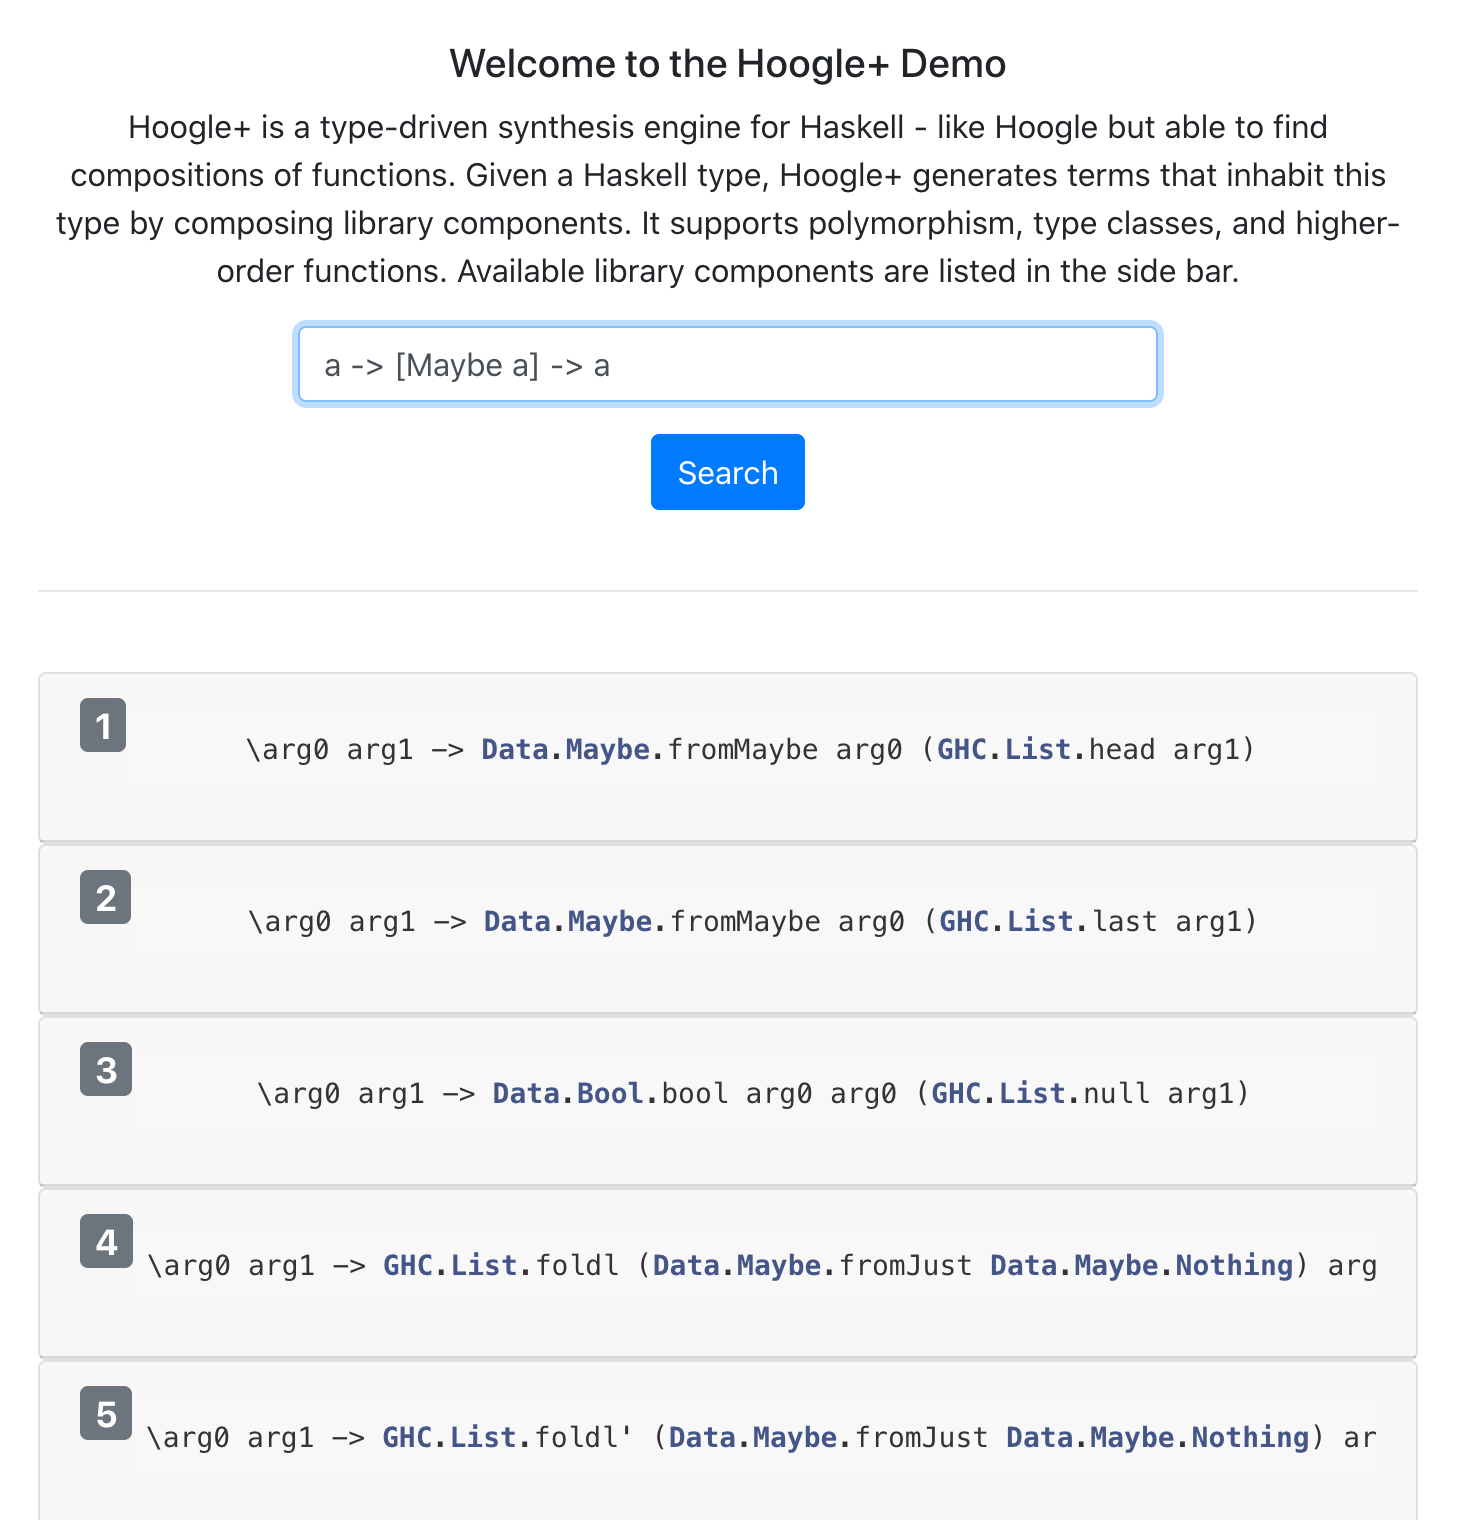
\includegraphics[width=\textwidth]{method/control-ui.png}
        \caption{Control treatment, no examples}
    \end{subfigure}%
    ~
    \begin{subfigure}[t]{0.5\textwidth}
        \centering
        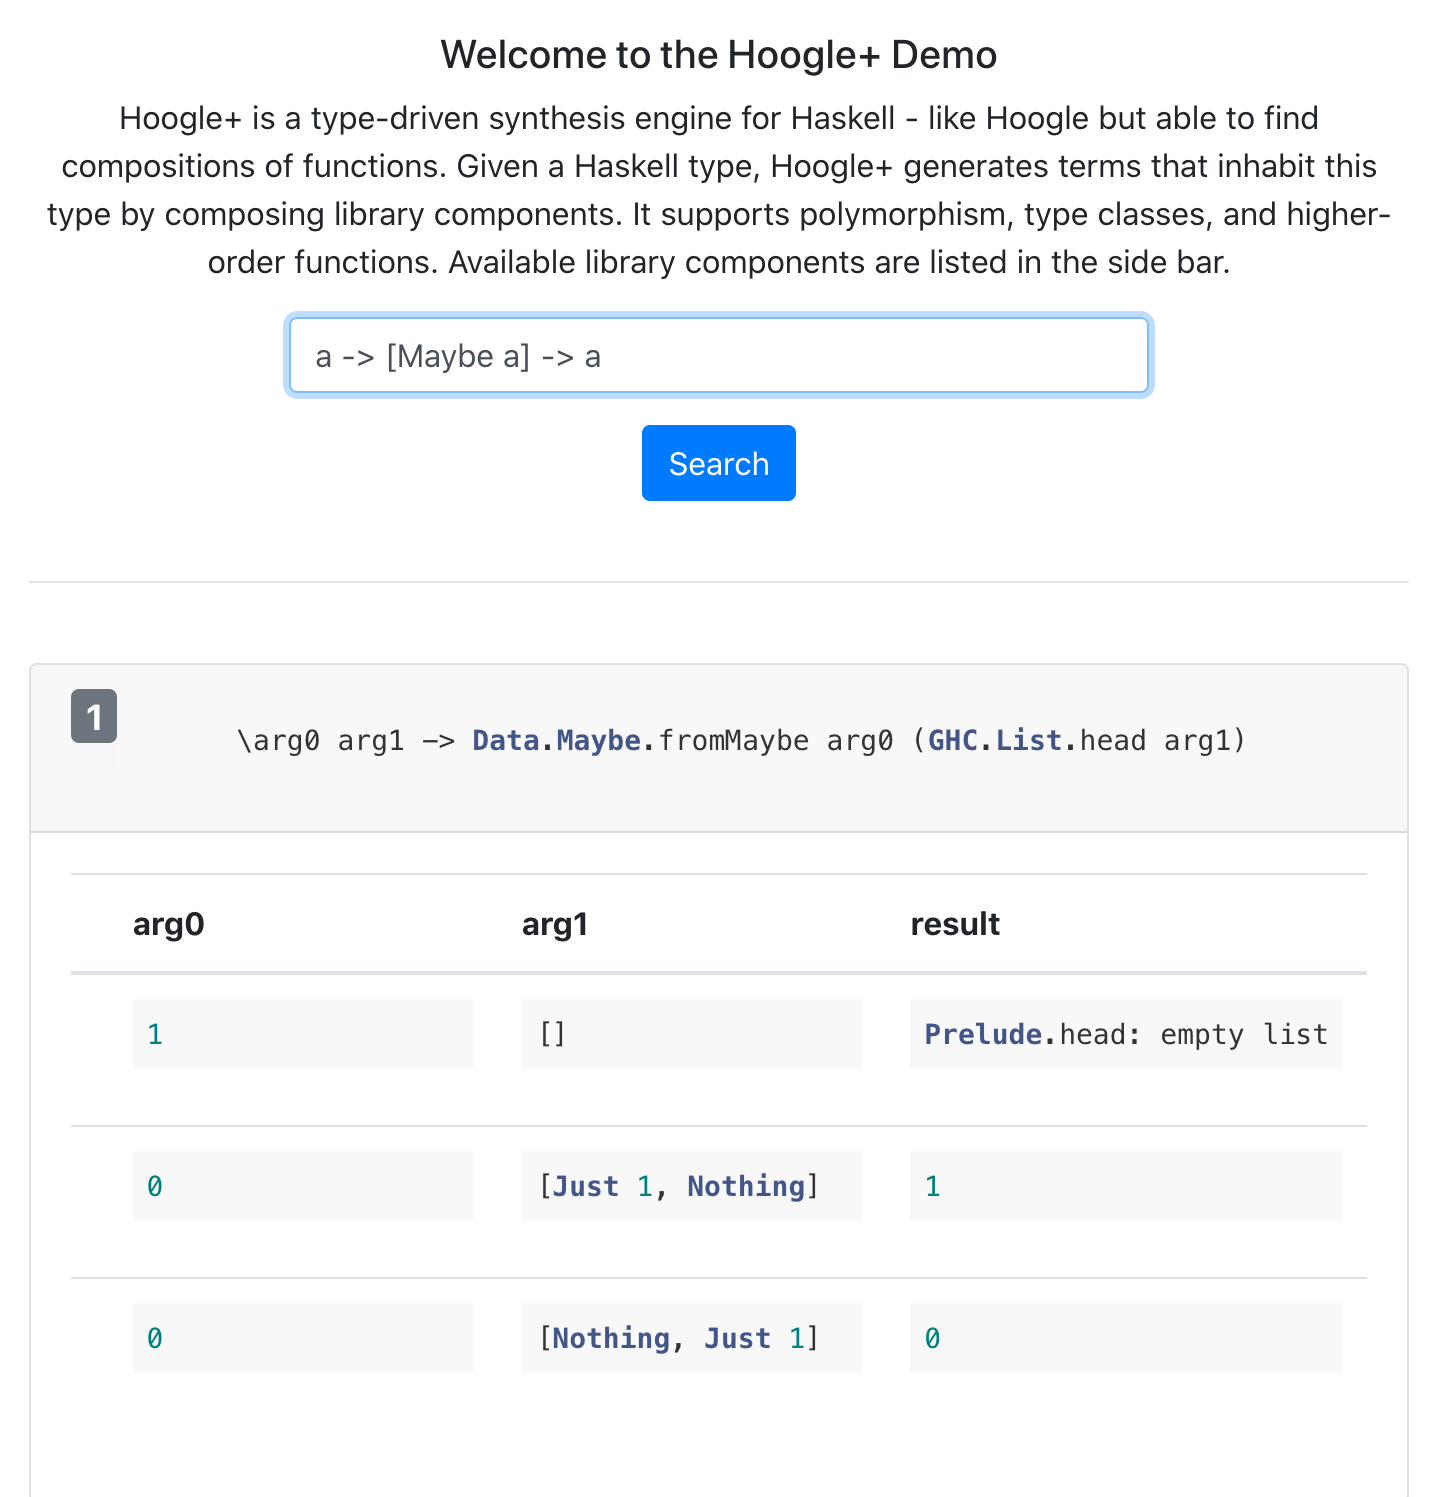
\includegraphics[width=\textwidth]{method/treatment-ui.png}
        \caption{Experimental treatment, examples}
    \end{subfigure}
    \caption{Each participant received one of the two treatments for the duration of the study.}
\end{figure*}

\section{Results}
\begin{figure*}[ht]
  \centering
  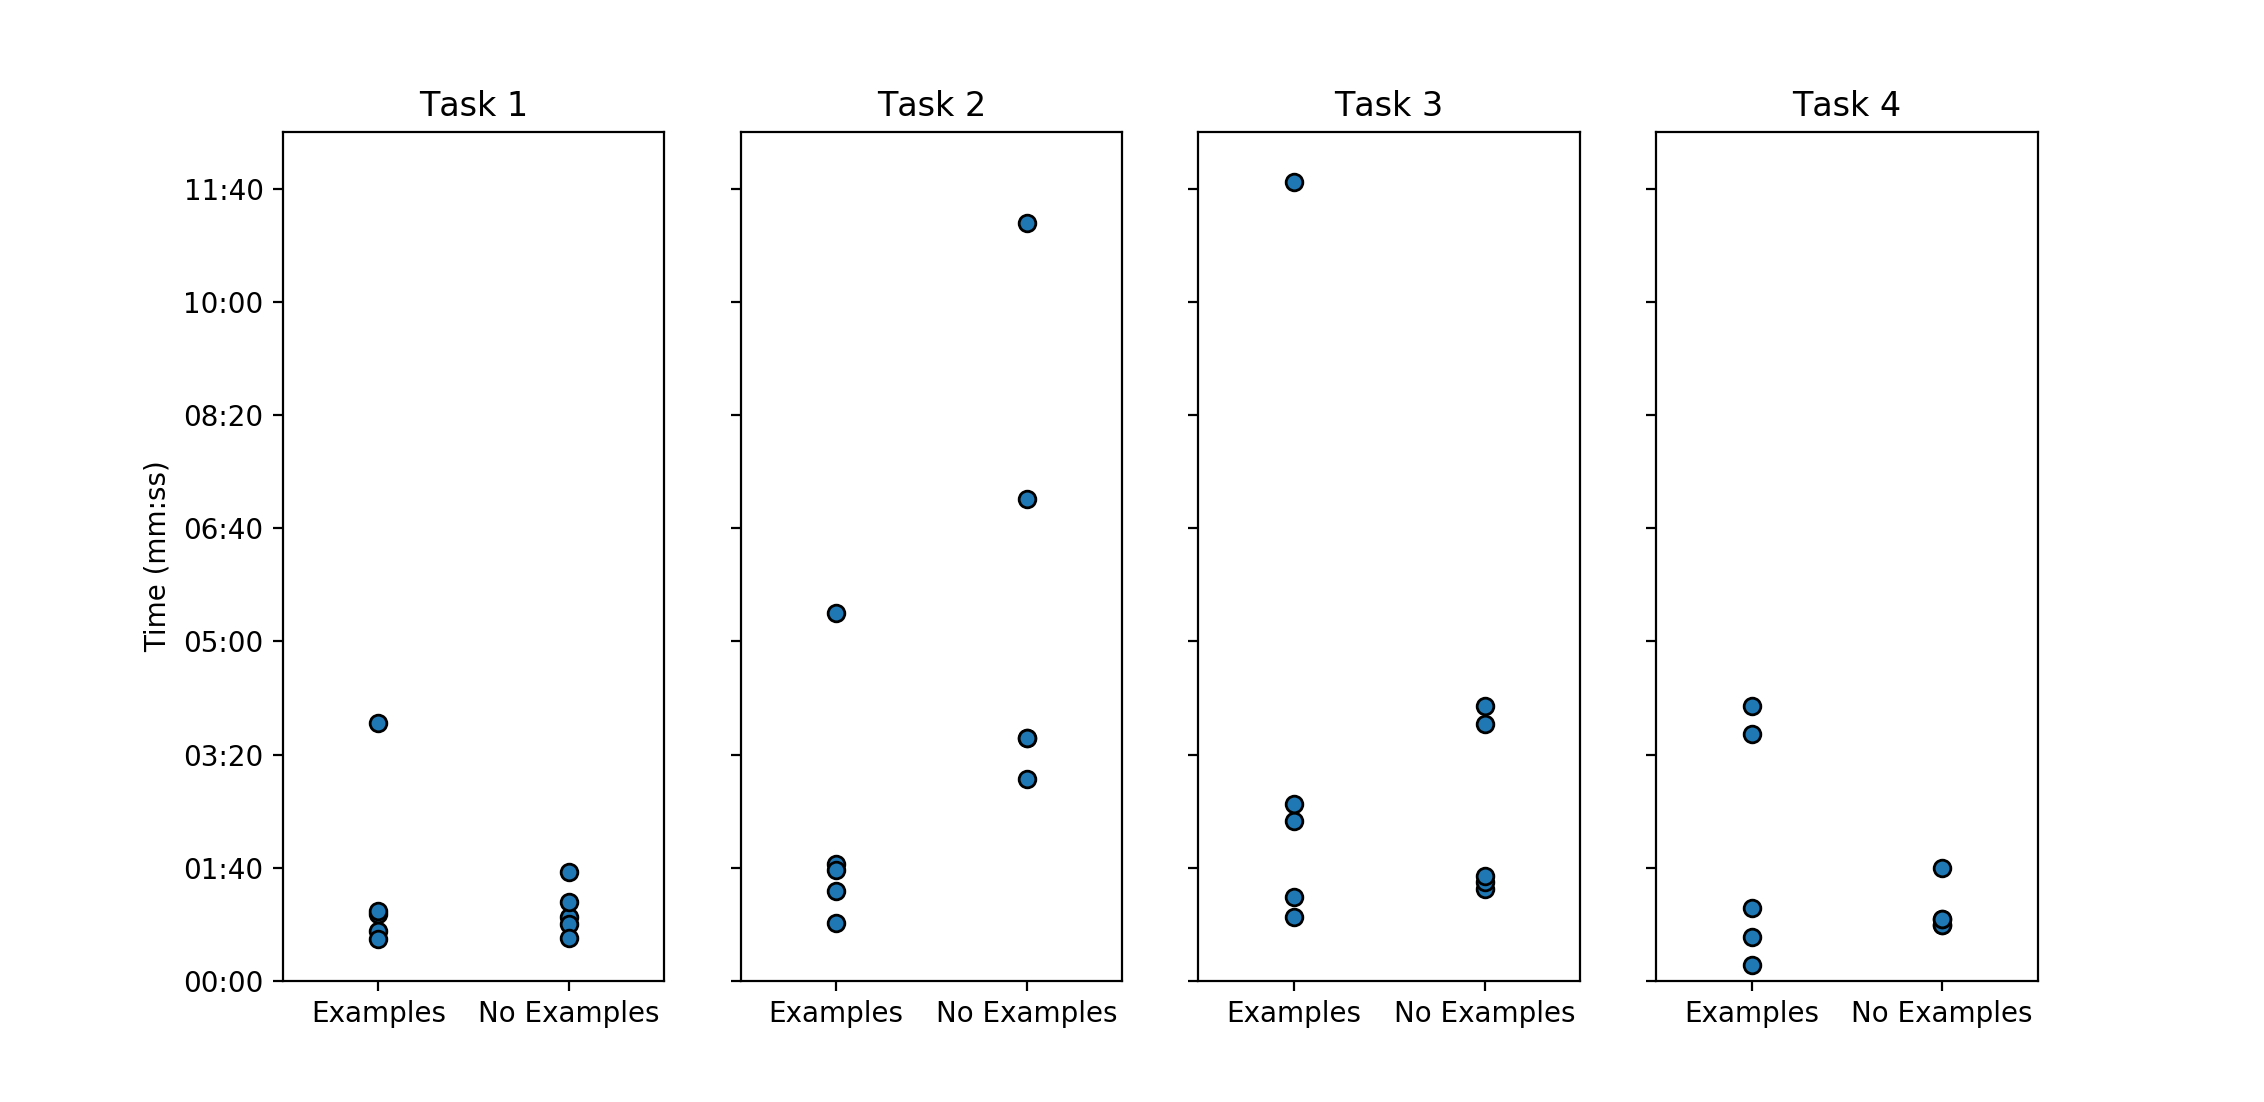
\includegraphics[width=\textwidth]{results/task_points.png}
  \caption{
    Examples did not noticeably affect time-to-completion, except in Task 2
    where the effect is dramatic.
  }
  \label{fig:data-points}
\end{figure*}
\subsection{Time-to-correct solution}
Cumulatively, across the four tasks, we did not observe a significant change
in the time-to-correct solution.
%
A Wilcoxon Rank-Sum test, performed on the aggregate of per-task rankings,
yielded a confidence interval of $p=0.14$.
%
Performing rank-sum of ranks is an especially conservative test, because it weighs
per-task rankings equally, regardless of the absolute times or relative
difficulty of tasks.

Although the results do not indicate a change across the board, our data shows a dramatic
speedup for the example group in Task 2 (see Figure~\ref{fig:data-points}).
%
This may indicate that certain tasks benefit from examples while others do not.
%
We discuss this more thoroughly in Section~\ref{sec:discussion}

\subsection{Incorrect selections}
When participants made an incorrect selection, they were allowed to keep
selecting until they found the correct program.
%
This happened 3 times in the \noexamples group and 5 times in the example group.
%
In the example group, a single participant made 3 incorrect guesses on a
single task.
%
This participant was also the only one who ranked their Haskell knowledge as a 1 out of 5.
%
Furthermore, the incorrect selections contained incorrect input/output pairs.
%
With these anomalies in mind, we don't believe this study has determined a definitive answer
on the relationship between examples and error rates.

\subsection{Interpreter usage}
In the \noexamples group, participants made a median of 6 type queries,
executed 3 subexpressions, and ran 3 full candidates across all 4 tasks.
%
In the \examples group, however, participants made a median of 0 queries of any kind.
%
It's clear that, introducing examples reduced participants reliance on the
interpreter to gather information.

% Figures.

\section{Discussion}

Discuss.

\section{Future Work}
\label{sec:future}

F U T U R E

\section{Conclusion}

We have shown an experimental setup to suss out when input-output examples help
users in a type-directed synthesis environment.
%
Overall our results did not show a statistical significance ($p = 0.14$);
however, we did find some interesting data points for further research.
%
Specifically, one task did conclude a statistically significant result ($p =
0.03$), Task 2.
%
We offered a theory explaining it and future experiments that could falsify our
claim.
%
We found that users did rely on an interpreter more in the absence of examples
to offer a "feel" for the candidate programs.


%%
%% The next two lines define the bibliography style to be used, and
%% the bibliography file.
\bibliographystyle{ACM-Reference-Format}
\bibliography{bib}

%%
%% If your work has an appendix, this is the place to put it.
\appendix

\end{document}
\endinput
%%
%% End of file `sample-sigchi.tex'.
